%!TEX program = xelatex
\documentclass[11pt,a4paper]{article}

% ── Packages ──
\usepackage[margin=0.7in]{geometry}
\usepackage{xeCJK}
\usepackage{fontspec}
\usepackage{titlesec}
\usepackage{enumitem}
\usepackage{hyperref}
\usepackage{xcolor}
\usepackage{graphicx}
\usepackage{wrapfig}
\usepackage{tabularx}
\usepackage{fancyhdr}

% ── Fonts ──
\setCJKmainfont{AR PL SungtiL GB}[BoldFont=AR PL KaitiM GB]
\setmainfont{DejaVu Sans}[BoldFont=DejaVu Sans Bold, ItalicFont=DejaVu Sans Oblique]

% ── Colors ──
\definecolor{primary}{RGB}{31, 78, 121}
\definecolor{accent}{RGB}{89, 89, 89}

% ── Hyperlink ──
\hypersetup{colorlinks=true, linkcolor=primary, urlcolor=primary}

% ── Section Formatting ──
\titleformat{\section}{\Large\bfseries\color{primary}}{}{0em}{}[\titlerule]
\titleformat{\subsection}{\large\bfseries}{}{0em}{}
\titleformat{\subsubsection}[runin]{\bfseries}{}{0em}{}

\titlespacing*{\section}{0pt}{12pt}{6pt}
\titlespacing*{\subsection}{0pt}{10pt}{4pt}

% ── List Style ──
\setlist[itemize]{leftmargin=1.2em, itemsep=1pt, parsep=0pt, topsep=2pt}

% ── Remove page number ──
\pagestyle{fancy}
\fancyhf{}
\renewcommand{\headrulewidth}{0pt}
\fancyfoot[C]{\thepage}

% ── Custom Commands ──
\newcommand{\stage}[3]{%
  \vspace{8pt}
  \noindent\textbf{\color{primary}#1} \hfill \textcolor{accent}{#2}\\[2pt]
  \textit{#3}
  \vspace{4pt}
}

\newcommand{\projectblock}[1]{%
  \vspace{4pt}\noindent\textbf{#1}\vspace{2pt}
}

% ══════════════════════════════════════════
\begin{document}

% ── Header ──
\begin{center}
  \begin{minipage}[c]{0.75\textwidth}
    \centering
    {\LARGE\bfseries 邵正悦 \quad Zhengyue Shao}\\[6pt]
    {\large Senior Android Platform Engineer \textperiodcentered{} Microsoft}\\[4pt]
    \textcolor{accent}{\href{mailto:zheshao@microsoft.com}{zheshao@microsoft.com}}
  \end{minipage}%
  \hfill
  \begin{minipage}[c]{0.2\textwidth}
    \raggedleft
    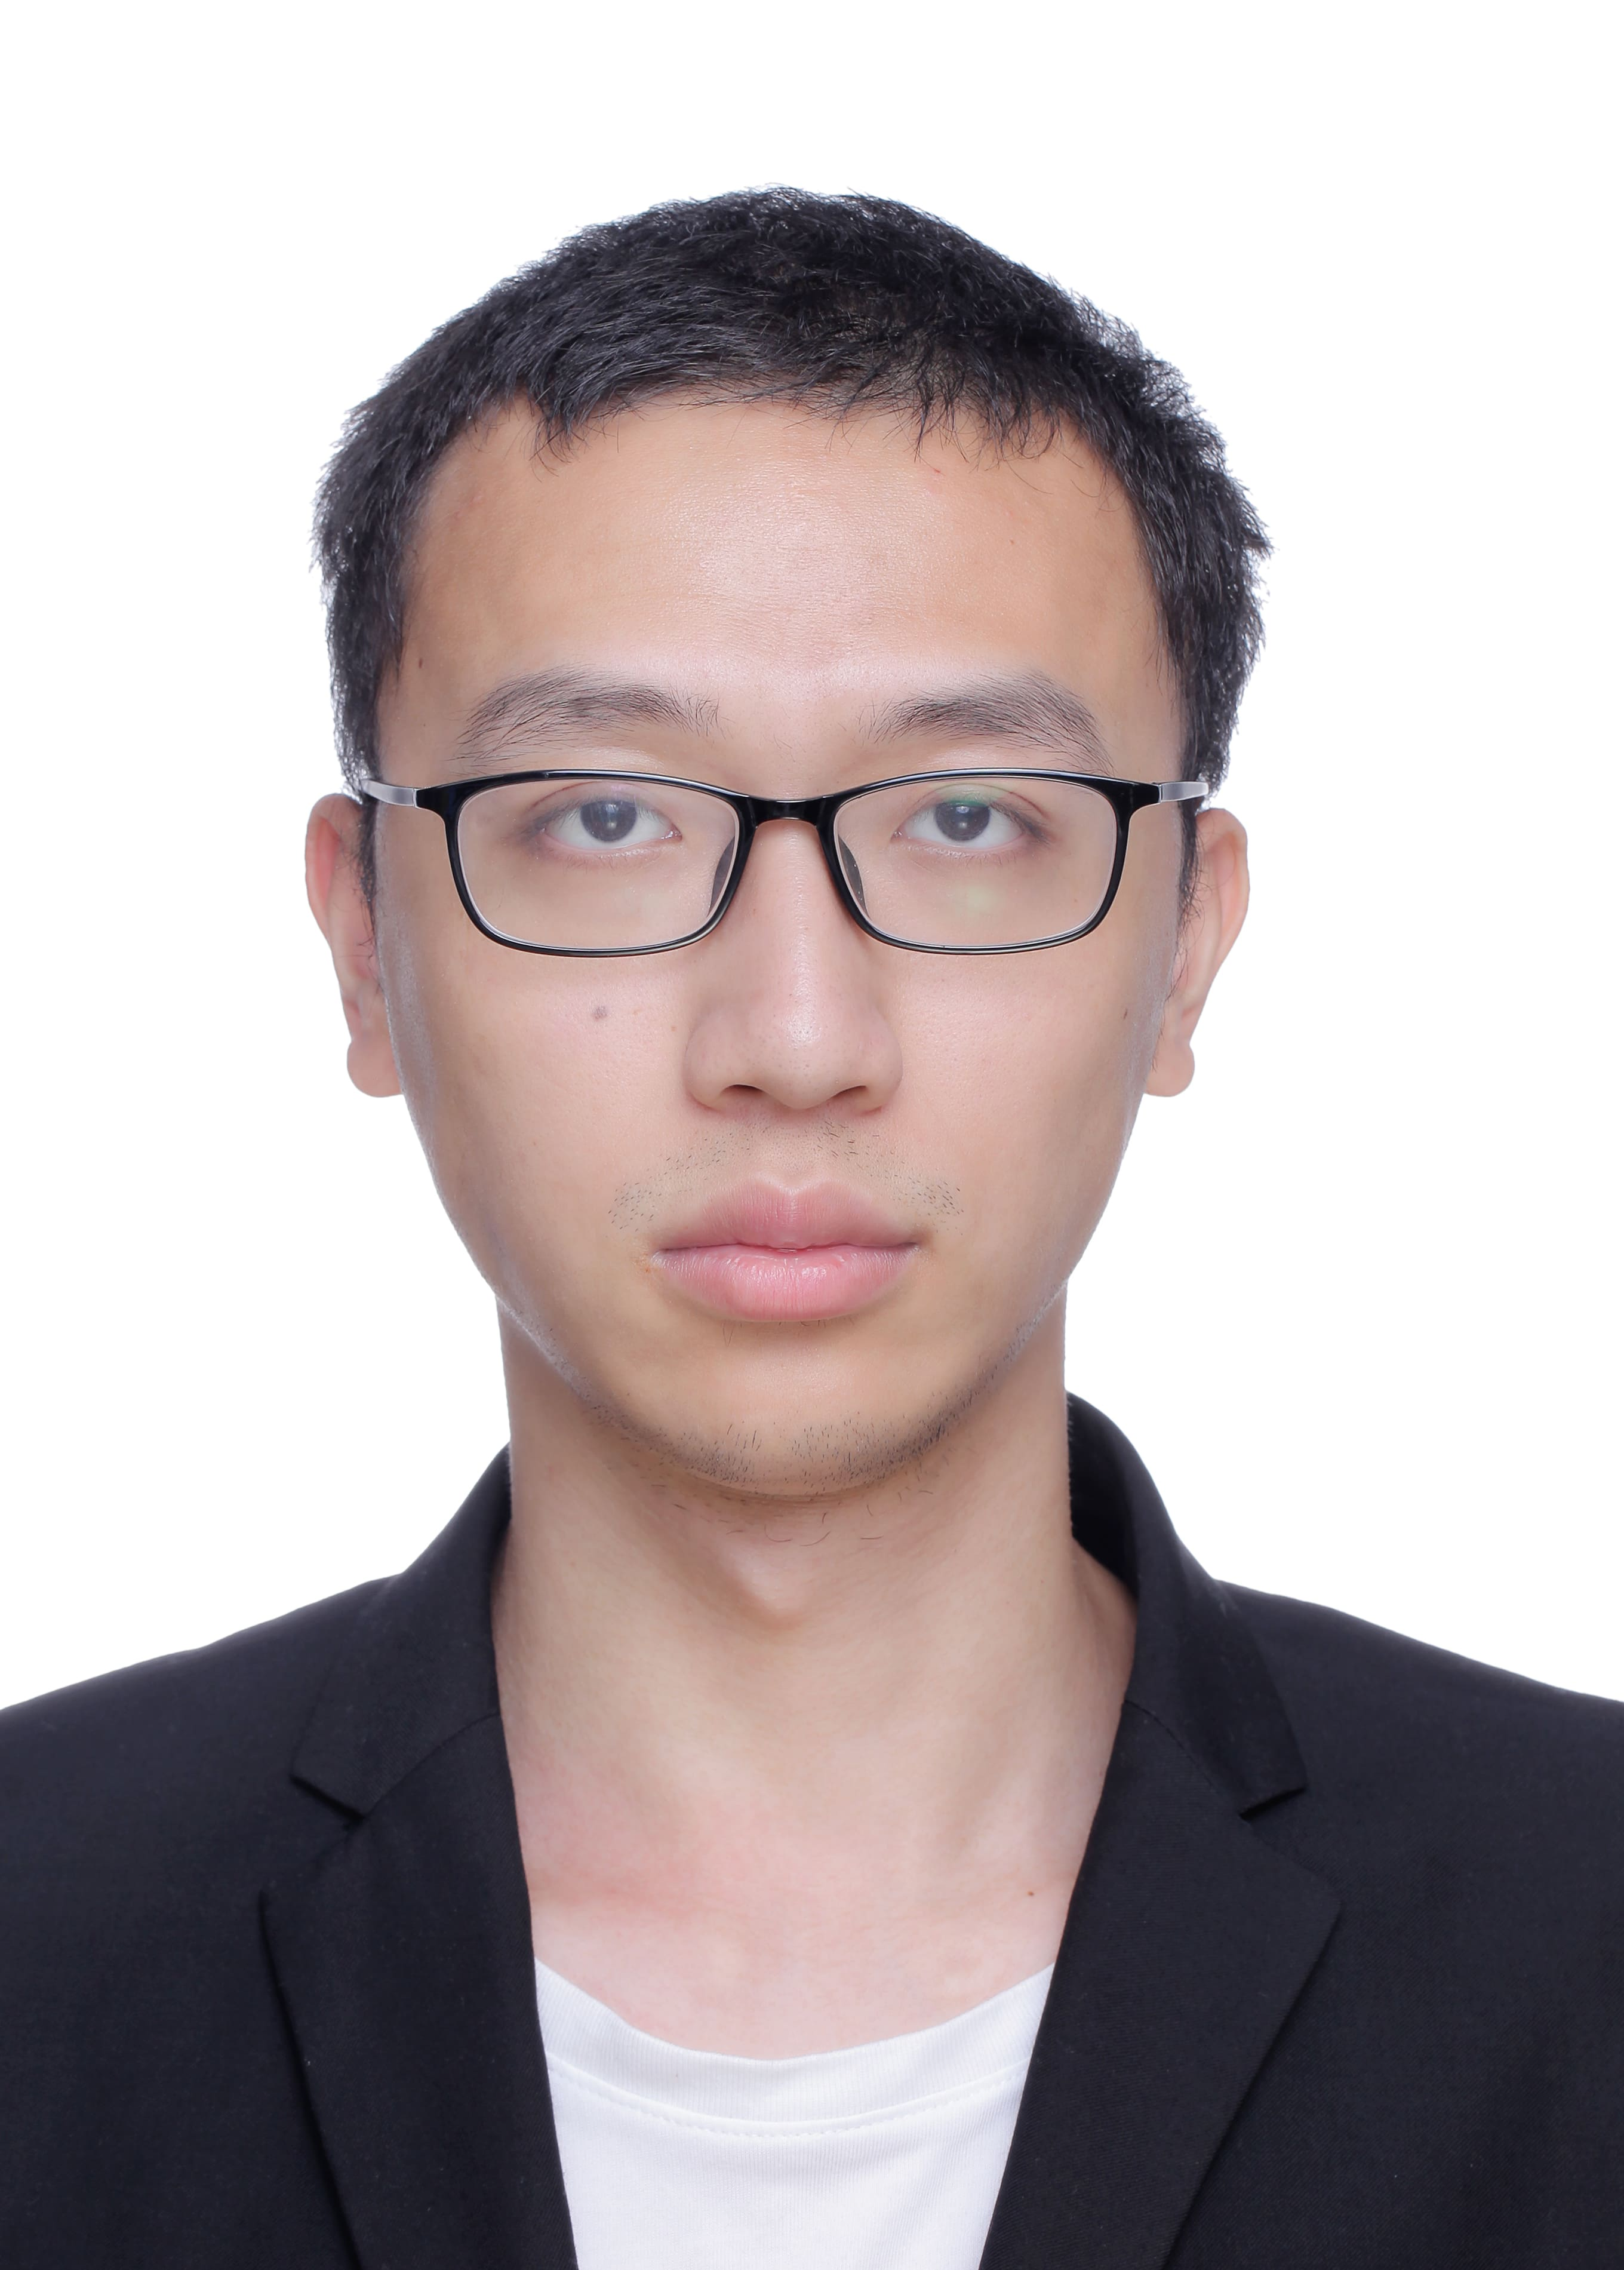
\includegraphics[width=2.8cm]{photo.jpg}
  \end{minipage}
\end{center}

\vspace{-2pt}

{\small
8+ 年 Microsoft 移动端平台工程经验，专注 Android 架构、SDK/Runtime 设计与 AI 产品集成。
技术主线从构建基础设施到语音助手到会议智能平台到 M365 Copilot 移动端 Runtime，
是 Microsoft 365 Copilot Mobile Runtime 的核心基础设施工程师之一。
}

% ══════════════════════════════════════════
\section{工作经历}

\noindent
\textbf{\large Microsoft} \hfill Software Engineer 2 \quad $|$ \quad 2017.06 -- 至今

% ── Copilot Mobile Runtime ──
\stage{M365 Copilot Mobile Platform / Runtime}{2024 -- 至今}
{负责 OneCopilotMobile (OCM) Android SDK 架构与平台工程，SDK 统一服务于 OfficeMobile、Outlook、Teams 等宿主应用，覆盖数亿用户。}

\begin{itemize}
  \item 设计移动端 AI Context Pipeline，将宿主应用的邮件/文档/选中内容标准化为结构化上下文，注入 Copilot 推理链路，实现 AI 上下文与 UI 层的解耦
  \item 负责 Copilot Runtime 核心基础设施：配置管理、服务路由、Feature Gate 灰度体系、模型切换等，支撑 GPT-5 集成与下一代富响应渲染
  \item 参与实时语音 AI 链路建设，优化连接预热延迟，修复异步状态竞态，保障生产环境可靠性；作为 Reliability Incident Owner 处理跨产品线生产事故
  \item 设计合规性双通道路由架构，为 WebSocket 通信引入企业级安全拦截（SSL Pinning / DLP / 审计），消除合规盲区
  \item 设计并交付图片上传合规流程与声明式授权拦截，平衡产品速度与隐私合规要求
  \item 负责 SDK 版本发布、宿主集成支持、跨模块兼容性维护与 Feature Flag 生命周期管理
\end{itemize}

% ── Teams MeetApp ──
\stage{Teams MeetApp — AI 会议智能平台}{2022 -- 2024}
{负责 MeetApp 全栈开发（React/TypeScript），为 Teams Desktop 用户提供 AI 增强的会议管理体验。}

\begin{itemize}
  \item 从零构建 MeetApp 核心架构：API 客户端、会议分类视图（Upcoming / Recent / Missed）、AI 会议摘要导航系统
  \item 设计并实现 MeetApp 内 Copilot 入口，集成 BizChat 对话流与跨会议 AI 摘要生成
  \item 构建实时调试工具与性能遥测体系，排查内存泄漏、导航延迟等复杂问题，驱动数据化性能优化
  \item 负责多轮 Feature Flag 灰度发布、无障碍适配与 Channel Meeting 等产品迭代
\end{itemize}

% ── Voice / Cortana ──
\stage{语音助手与对话式 AI 体验}{2019 -- 2022}
{先后在 Outlook PME 和 Teams Cortana 团队，负责 Play My Email、Catch Me Up 等语音驱动生产力功能的 Android 端开发。}

\begin{itemize}
  \item 从 POC 到 GA 全程主导 Catch Me Up 在 Teams Android 的集成，设计 React Native 原生桥接层，实现语音唤醒、TTS 播放、消息 triage 等完整交互链路
  \item 在 Outlook 实现 TTS 流式邮件播报，开发语音指令回复/标记/归档等 hands-free 邮件处理能力
  \item 主导 Hermes 引擎迁移与 SDX 架构迁移，支持 Gov Cloud 部署，提升运行时性能
\end{itemize}

% ── Build Infra ──
\stage{SharePoint 构建基础设施}{2017 -- 2019}
{负责 SharePoint Online 构建系统现代化，支撑大规模 Monorepo 的构建效率与稳定性。}

\begin{itemize}
  \item 主导 Domino (BuildXL) 构建引擎迁移，优化增量构建管道，负责跨分支集成与构建中断响应
\end{itemize}

% ══════════════════════════════════════════
\section{教育背景}

\noindent
\textbf{浙江大学} \hfill 2014 -- 2017\\
计算机科学与技术 硕士 \quad\textcolor{accent}{研究方向：移动安全、BYOD 访问控制}

\vspace{6pt}
\noindent
\textbf{南京航空航天大学} \hfill 2010 -- 2014\\
计算机科学与技术 学士 \quad\textcolor{accent}{（2009 年 NOIP 一等奖保送）}

% ══════════════════════════════════════════
\section{学术发表}

\begin{enumerate}[leftmargin=1.5em, itemsep=4pt]
  \item \textbf{RiskCog: Unobtrusive Real-Time User Authentication on Mobile Devices in the Wild}\\
    T.~Zhu, Z.~Qu, H.~Xu, J.~Zhang, \textbf{Z.~Shao} et al.\\
    \textit{IEEE Transactions on Mobile Computing}, 2019 \quad $|$ \quad \textbf{被引 92 次}

  \item \textbf{AppShield: Enabling Multi-entity Access Control Cross Platforms for Mobile App Management}\\
    Z.~Qu, G.~Guo, \textbf{Z.~Shao}, V.~Rastogi, Y.~Chen, H.~Chen, W.~Hong\\
    \textit{SecureComm 2016} (Springer LNCS) \quad $|$ \quad \textbf{被引 11 次}
\end{enumerate}

% ══════════════════════════════════════════
\section{技术技能}

\begin{tabularx}{\textwidth}{@{} >{\bfseries}l X @{}}
Android 平台  & Kotlin, Java, Jetpack Compose, Coroutines/Flow, Dagger/Hilt, OkHttp/WebSocket, Room, React Native \\[3pt]
架构与 SDK    & MVVM, Clean Architecture, SDK/Runtime 设计, 模块化, 依赖注入, Host/Plugin 架构, Feature Gate 体系 \\[3pt]
AI 与产品集成 & Copilot 集成, AI Context Pipeline, 语音交互 (TTS/AEC/KWS), 合规性 UX, 模型切换 \\[3pt]
工程实践      & Monorepo CI/CD, 构建系统, 性能遥测/Kusto, 灰度发布, 生产事故响应, 跨团队协作 \\
\end{tabularx}

\end{document}
